\chapter{ゴルフスイングのバイオメカニズム}
\section{バイオメカニクス}
バイオメカニクス(biomechanics)とは,生体に力が作用して起こる現象を取り扱う,力学の一分野であり,日本語では生体力学,あるいは生体機械工学とも呼ばれる.
バイオメカニクスでは,ヒトだけでなく動植物をはじめとするあらゆる生物を対象とし,対象の生物の器官系,器官,組織,細胞,遺伝子といった,各レベルまで扱う.
バイオメカニクスの歴史として,14世紀から16世紀に急速にヒトの内部の仕組みを知りたいという願望が増大し,その中でも,レオナルド・ダ・ビンチが人体解剖図を精密がしたことが有名である.

現在のバイオメカニクスの分野では,バイオメカニクスに関連した学問や分野が発展しており,解剖学,生理学,医用工学,人間工学,スポーツ工学,と言った分野は盛んであり,本研究もスポーツ工学の分野に位置づく.
%
\section{人体構造}
図\ref{基本的立位姿勢}は基本的立位姿勢を示す.
\begin{figure}
    \begin{center}
        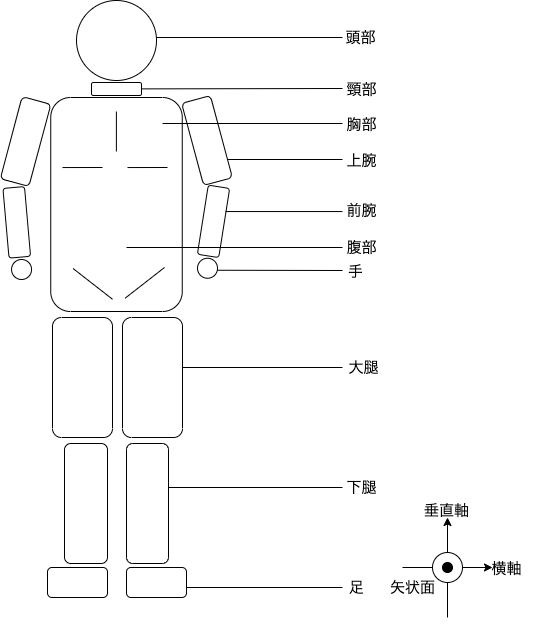
\includegraphics[width = 5cm]{./images/human_body.png}
        \caption{基本的立位姿勢}
        \label{基本的立位姿勢}
    \end{center}
\end{figure}
ヒトには,いくつかの部位のグループで呼ばれることがある.
一般に体幹と呼ばれるグループがあるが,
広い幅の意味を持つ体幹とは図\ref{基本的立位姿勢}より,頭部,頸部,胸部,腹部のグループであり,その中でも胸部,腹部のみでも体幹と呼ばれることがある.
上腕,前腕,手の三部位を総称し上肢と呼び,大腿,下腿,足の三部位を総称し下肢と呼ぶ.
また,上肢,下肢を総称し体肢,四肢と呼ばれることがある.
% 本研究もこの名称に従い,部位の名称を扱う.

次に,運動の基準とする軸について説明する.
図\ref{基本的立位姿勢}より,床と頭部を結ぶ軸を垂直軸,床と左右に並行の軸を横軸,背面から前方方向への軸を矢状軸と呼ぶ.


% \section{関節}
% 本節ではヒトの関節名称を示す.
% \begin{figure}
%     \begin{center}
%         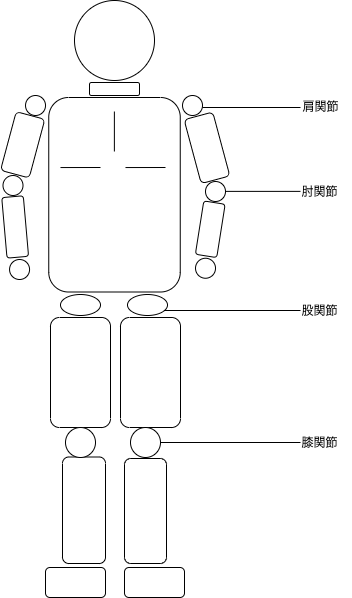
\includegraphics[width = 5cm]{./images/joint.png}
%         \caption{関節構造}
%         \label{関節構造}
%     \end{center}
% \end{figure}
% 図\ref{関節構造}の,

\section{人体の運動表現}
ヒトが運動する際に,その時の運動の表現は世界共通の表現がある.
本節では,日本整形外科学会の規則に則り,ヒトの運動表現について説明を行う.

ヒトには,屈曲/伸展,外転/内転,外旋/内旋の三種類の基本動作がある.
屈曲/伸展とは,横軸に並行な運動である.
一般に,頭部,胸部が前方に倒れる方向を屈曲,反対の動きを伸展と呼ぶ.
外転/内転とは,矢状軸に並行な運動である.
一般に,上肢を床と並行,矢状軸と直角になる運動を外転,反対の動きを内転と呼ぶ.
また,頸部,胸部,腰部は定義に則した運動に一致しないことから,側屈と呼ばれることがある.
外旋/内旋とは,垂直軸に並行な運動である.
一般に,前腕を床と並行かつ上腕と直角にした状態で,上体の方向に回転する運動を内旋,上体から離れるような回転を外旋と呼ぶ.
また,頸部,胸部,腰部は定義則した運動に一致しないことから,回旋や捻転と呼ばれることがある.

\section{ゴルフ}
%
現在,日本のゴルフはかなり盛んであり,プロゴルファーの松山や渋野が海外で活躍するのをきっかけに,全世代的に見ても流行の兆しがある.
特に,日本のゴルフ用品の市場規模は,世界二位の2000億円であり,ますます期待のスポーツである.

ゴルフの初心者等は,上達のためにスクールに通いインストラクターをつけ,最新の器具や設備,解析機器を使用して練習に励む動向がある.
特に現代の技術では,
ハイスピードカメラや高性能カメラを使用したモーションキャプチャを用いたゴルフスイング解析,
トラックマンを使用し飛球したゴルフボールの弾道の測定,
また,動画技術も向上したため様々な流儀のスイング解説がある.


\section{ゴルフスイング}
\section{ゴルフボールの弾道}
\section{ヘッドアップ動作}
\section{身体が開く動作}


